\documentclass[12pt]{article}
\usepackage[paperwidth=13.333in,paperheight=7.5in,margin=0in]{geometry}
\usepackage[T1]{fontenc}
\usepackage{lmodern}
\usepackage{amsmath,amssymb}
\usepackage{graphicx}
\usepackage{xcolor}
\usepackage{tikz}
\usepackage{helvet}
\renewcommand{\familydefault}{\sfdefault}
\pagestyle{empty}
\setlength{\parindent}{0pt}
\usetikzlibrary{positioning,calc,fit,backgrounds}
\definecolor{markovadd}{HTML}{4C78A8}
\definecolor{markovneural}{HTML}{E45756}
\definecolor{ctreegreen}{HTML}{54A24B}
\definecolor{guideorange}{HTML}{F58518}
\definecolor{softgray}{HTML}{F4F6F8}
\definecolor{midgray}{HTML}{D9DEE3}
\newcommand{\slidebox}[4]{
  \node[anchor=north west, rounded corners=7pt, draw=#1!70!black, fill=#1!8, line width=0.9pt, inner sep=10pt,
        align=left] at #3 {\parbox{#2}{\raggedright #4}};
}
\begin{document}
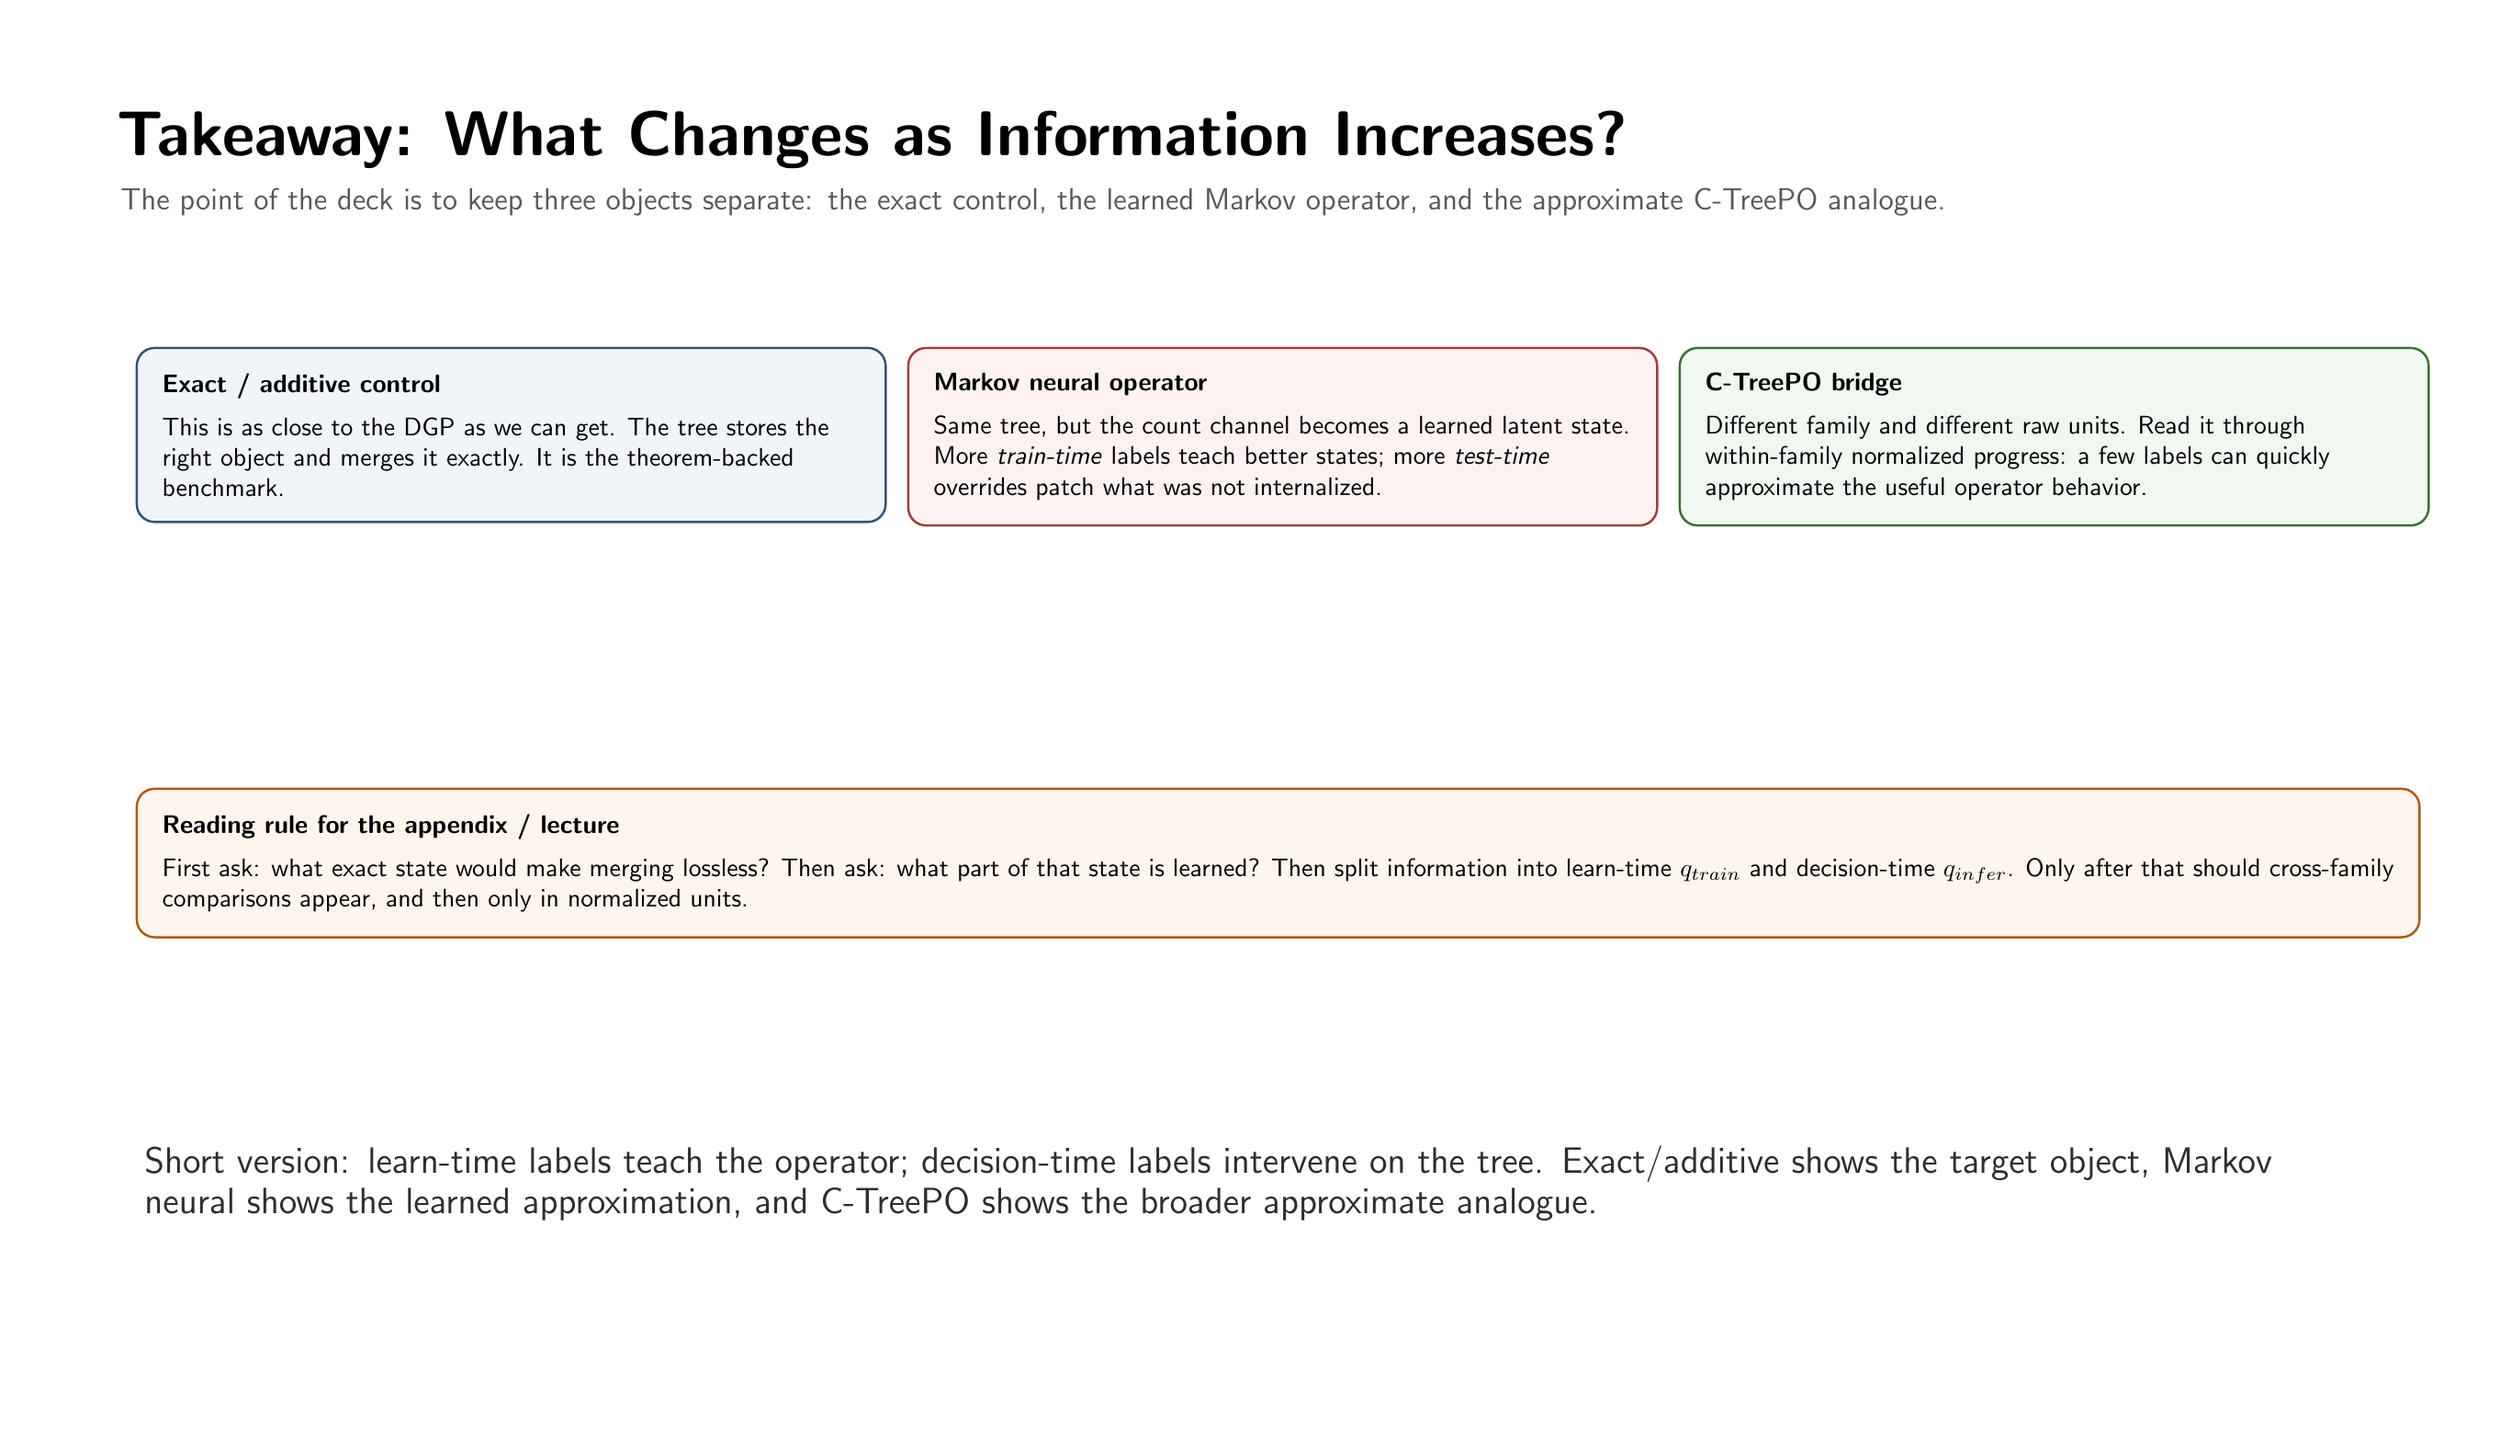
\begin{tikzpicture}[x=1in,y=1in]
\useasboundingbox (0,0) rectangle (13.333,7.5);

\node[anchor=north west, font=\bfseries\fontsize{26}{28}\selectfont] at (0.45,7.08) {Takeaway: What Changes as Information Increases?};
\node[anchor=north west, text=black!65, font=\fontsize{13}{15}\selectfont, text width=12.15in] at (0.47,6.66) {The point of the deck is to keep three objects separate: the exact control, the learned Markov operator, and the approximate C-TreePO analogue.};
\slidebox{markovadd}{3.8in}{(0.60,5.75)}{\bfseries Exact / additive control\\[0.45em]\mdseries This is as close to the DGP as we can get. The tree stores the right object and merges it exactly. It is the theorem-backed benchmark.}
\slidebox{markovneural}{3.8in}{(4.80,5.75)}{\bfseries Markov neural operator\\[0.45em]\mdseries Same tree, but the count channel becomes a learned latent state. More \emph{train-time} labels teach better states; more \emph{test-time} overrides patch what was not internalized.}
\slidebox{ctreegreen}{3.8in}{(9.00,5.75)}{\bfseries C-TreePO bridge\\[0.45em]\mdseries Different family and different raw units. Read it through within-family normalized progress: a few labels can quickly approximate the useful operator behavior.}
\slidebox{guideorange}{12.15in}{(0.60,3.35)}{\bfseries Reading rule for the appendix / lecture\\[0.45em]\mdseries First ask: what exact state would make merging lossless? Then ask: what part of that state is learned? Then split information into learn-time $q_{train}$ and decision-time $q_{infer}$. Only after that should cross-family comparisons appear, and then only in normalized units.}
\node[anchor=north west, text width=12.0in, font=\fontsize{14}{16}\selectfont, text=black!82] at (0.60,1.45) {Short version: learn-time labels teach the operator; decision-time labels intervene on the tree. Exact/additive shows the target object, Markov neural shows the learned approximation, and C-TreePO shows the broader approximate analogue.};
\end{tikzpicture}
\end{document}
